\documentclass[a4paper,11pt]{article}
\usepackage[utf8]{inputenc}
\usepackage{amsmath}
\usepackage{amsfonts}
\usepackage{amssymb}
\usepackage{graphicx}
\usepackage[backend=biber]{biblatex}

\addbibresource{nn.bib}
\renewcommand\thesubsection{\alph{subsection}}


%opening
\title{Delay-dependent synchronized traveling waves in neural columns}
\author{Vince Baker, advisor: Dr. Luis Cruz Cruz\\ Drexel University Department of Physics}

\begin{document}

\maketitle

\begin{abstract}
Cortical traveling waves have been observed in vivo and in simulations of recurrent networks.
These traveling waves explain various features of cortical dynamics including spike timing variability and correlated fluctuations in membrane potential.
In this work we examine the firing dynamics of neural column structures similar to those found in the cortex.
We find that traveling waves are evoked by random background stimulus in networks with distance-dependent connectivity.
We also demonstrate that the propagation velocity of the action potentials effects wave formation.
In particular, networks with propagation time porportional to inter-neuron distance exhibit traveling waves while otherwise identical networks with constant or random propagation time do not show synchronization.

\end{abstract}

\section{Introduction} 
Synchronization in networks of neurons may arise from a combination of the network topology, interaction strengths, stimulus properties and neuron and synapse dynamics.
Propagating waves have been observed on multiple scales in different regions of the brain \cite{muller2018}.
These waves have been proposed to explain irregular neural dynamics \cite{keane2015} and various computational roles \cite{muller2018}. 
\\
Cortical topology is organized into column structures. 
The basic unit is the microcolumn or minicolumn \cite{cruz2005}, a structure of about 100 neurons that is a few tens of microns thick and several millimeters long oriented perpendicular to the cortical layers.
The cortex is further organized into larger columnar structures a few hundred microns thick. 
\\
We study the emergence of traveling waves in columnar structures with biologically plausible neural parameters and connectivity.

\section{Methods}
We simulated the dynamics of a small neural column to explore neuron synchronization.
Our network geometry is based on the model presented in \cite{markram1998}.
The neural column is composed of 135 neurons on a unit column, 3x3 neurons wide and 9 neurons high as shown in figure \ref{fig:column_structure}.
\begin{figure}[ht]
 \caption{Column structure used in this research, $\lambda=2$,$C=1$,}
 \label{fig:column_structure}
 \centering
   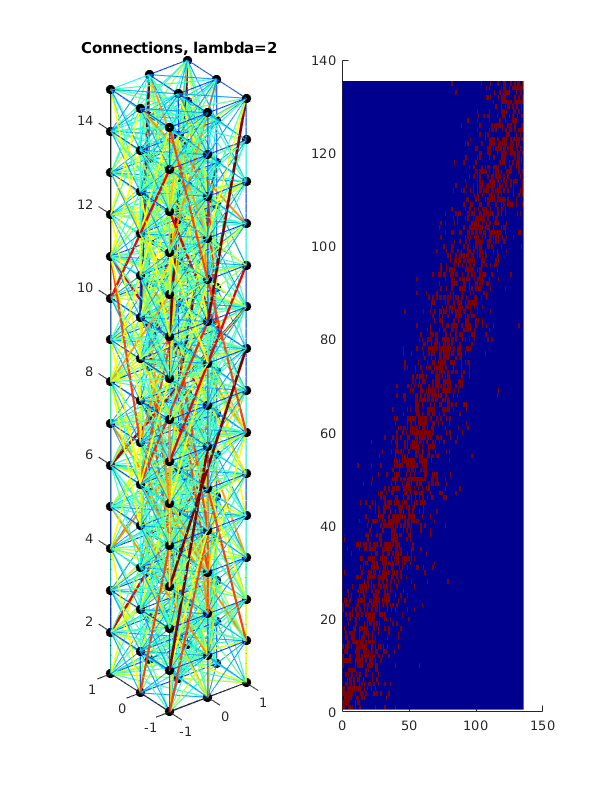
\includegraphics[width=0.48\textwidth]{fig/lambda2}
\end{figure}
The neurons are connected according to a distance-based rule:
\begin{align}\label{eq:connectivity}
 P_{a,b} &= C \times e^{-(D(a,b)/\lambda)^2}
\end{align}
We model the neurons using the Izhikevich model \cite{izhikevich2003} to allow us to explore the neural dynamics.
The Izhikevich model uses two coupled differential equations with two variables and four parameters:
\begin{align}
 v^\prime &= 0.04v^2+5v+140-u+I\\
 u^\prime &= a(bv-u)\\
 \text{if } &v>30: v\leftarrow c, u\leftarrow u+d
\end{align}
This is a simplified model of a two-dimensional dynamical system.
This model has been used to reproduce common neural firing patterns.
There is MATLAB code available that implements this neural model with fixed, single-time-step action potential propagation.
We enhanced the available MATLAB code for the Izhikevich model to incorporate propagation time between the neurons through the use of a delay buffer.
This allowed us to study the temporal effects of action potential propagation times.
We simulate networks with both random propagation delays and propagation delays that depend on the distance between the neurons.
\\
We capture the firing events from all neurons in each simulation.
We then perform a spatial clustering operation to identify spatiotemporal regions with a high firing density.
This clustering operation removes random background firing activity.
We then identify and label the traveling wave structures that evolve over time.
\begin{figure}[ht]
 \caption{A: Neuron firings in a column with 30\% excitatory neurons. B: The resulting cluster points (black) and an example of a labeled wave (red).
          C: Neuron firings in a column with 80\% excitatory neurons. D: The resulting cluster points (black) and an example wave (red).}
 \label{fig:wave_analysis}
 \centering
   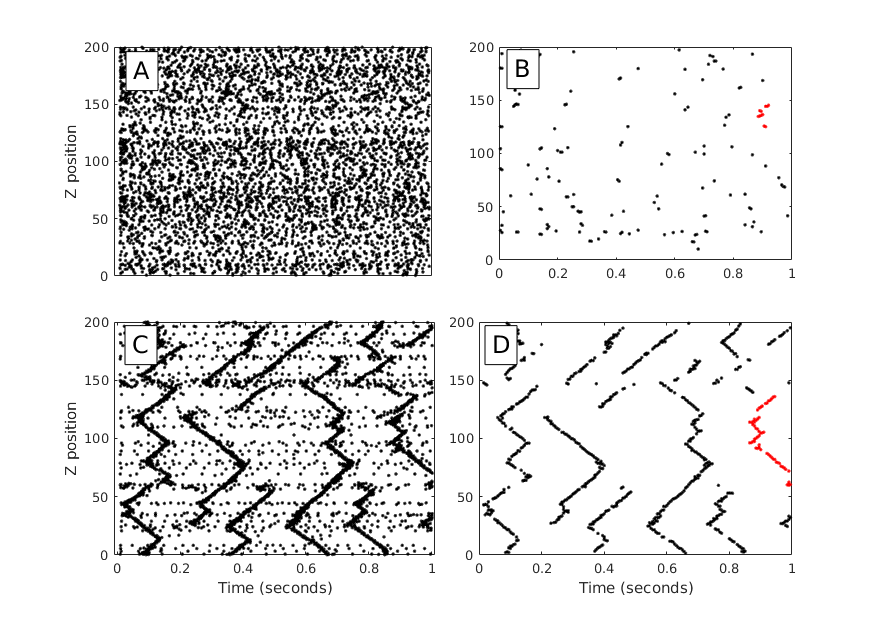
\includegraphics[width=\textwidth]{fig/WaveAnalysisExample}
\end{figure}


\section{Results}
Traveling wave behavior emerges when the excitatory neuron fraction is between 50\% and 98\%.
\begin{figure}[ht]
 \caption{Traveling wave statistics for columns with differing excitatory/inhibitory balance. 
	  For columns with <50\% excitatory neurons no waves are observed. 
	  Top: as the percent of excitatory neurons increases, the number of firing events per wave increases. 
	  Middle: The fraction of the total neural firings that are part of traveling wave structures increase with increasing excitation.
	  Bottom: The propagation velocity of the waves does not show dependence on the excitatory/inhibitory balance.}
 \label{fig:excitatory_effect}
 \centering
   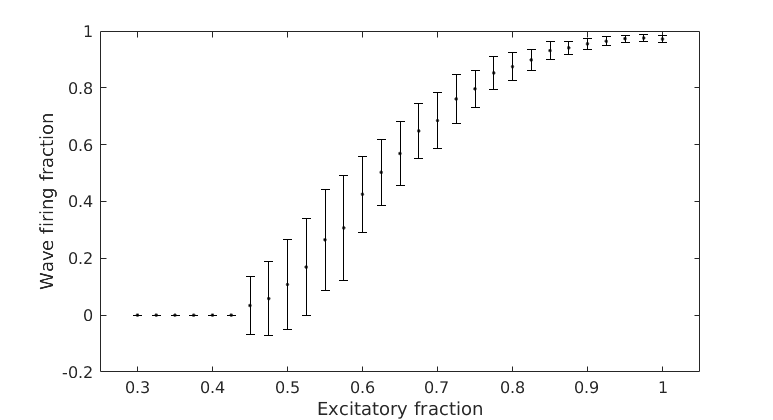
\includegraphics[width=\textwidth]{fig/ExcitatoryWaves}
\end{figure}
\\
We simulated various networks with random delays, fixed delays and distance-dependent delays.
We found that only distance-dependent delay networks produced traveling waves.


\section{Future work}


\clearpage
\printbibliography

\end{document}
